\section{Schedule and Budget}

The proposed schedule and estimate of costs for the 35t prototype RCE-based DAQ is shown in Fig. \ref{fig:budget35t}.  

\begin{figure}[htb]
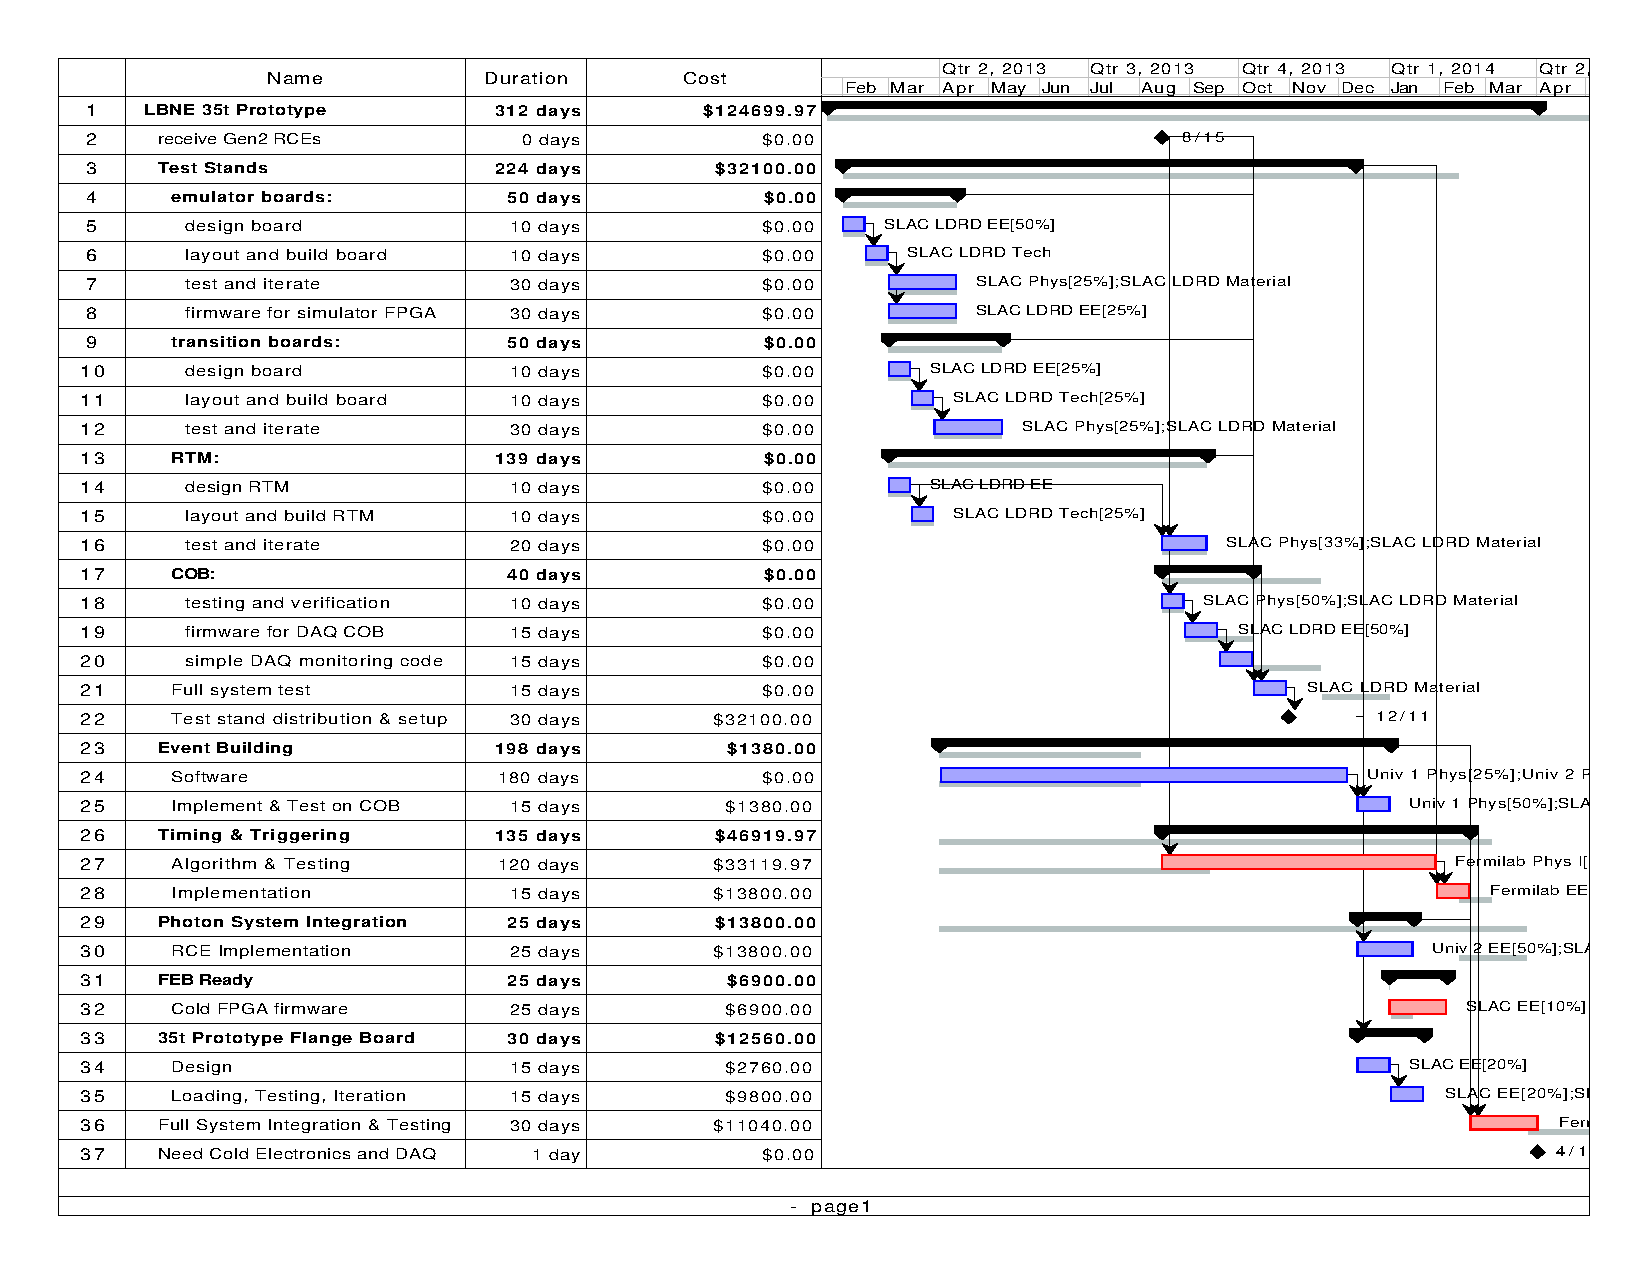
\includegraphics[scale=0.8,angle=90]{project-gantt.pdf}
\caption{Schedule and budget for the 35t RCE-based DAQ.}
\label{fig:budget35t}
\end{figure} 

This proposal uses the Gen-3 COBs which are expected to be available in August  (???) at the latest.  The Gen-3 COBs will use the Virtex ZYNQ SoC (series-7) which has many advantages over the series-5 previously used.  Probably the most important feature for our purposes is that it is distributed with with a Linux distribution.  This makes software development much simpler; we can develop our algorithms in C++ on a Linux PC and simply copy them directly to the RCEs.  While there is overhead involved with running Linux (and it cannot come near the speed of running algorithms in firmware), we expect that it will be fast enough for the few hundred Hz trigger rates expected in the 35t prototype.  

The budget includes 4 DAQ test stands composed of a 2-slot ATCA crate (with power), a COB and RTM, a simplified flange board, and an emulation board.  The emulation board will consist of a Virtex-5 FPGA programmed to output data with format and rate  similar to that expected from the TPC FEB and transmit it to the flange board via copper.  The test stands will allow us to develop the DAQ system at places other than at SLAC.  One of these test stands can likely be used for the 35t DAQ system.    Much of the development needed to get the first test-stand working will be covered under a SLAC LDRD so, for project purposes, is considered to be available at no cost.  

There are a number of tasks necessary for the complete working system that can be done semi-independently of the full ATCA-based DAQ.  Preliminary work on some of these items can start immediately on test boards or PCs which is advantageous because we don't expect to receive the Gen-3 boards until August.  All of the tasks listed can be performed by non-SLAC universities or labs with a low-level of SLAC support.  
\begin{itemize}
\item Timing/Trigger:  The external clock and trigger must be integrated into the RTM/COB and distributed to the FEBs.  Much of this work likely requires a COB.  Details on the clock and trigger signals may be necessary for RTM design.   
\item Event Building:  If desired, some level of event building can be performed in the COBs before sending to the PC farm.  This work can be done by a physicist and can be started at any time with C++ code on a Linux PC and be transfered to the RCEs when ready.   
\item PGP Implementation on FEB:    Once the FEB is laid out,  we can used a PCIe-based PGP card to program  the cold FPGA (up to timing/trigger, which will require the COB).  This task requires an EE.    
\item Photon System:  The output and timing/trigger needs will need more fleshing out.  This may require either a different RTM or flange board than the TPC.  The design of this can be done independently of the COB.  
\end{itemize}


%================
\begin{table}[tbh]
\begin{center}
\begin{tabular}{|l|c|c|}   
\hline \hline 
    & Hours  & Cost ($1k$) \\      
\hline
   Physicist           & XXXX&0 \\ 
   Engineer           & XXXX& XXXX\\ 
   Technician        & XXXX&XXXX \\ 
\hline \hline
\end{tabular}
\caption[]{Total number of work hours and assumed cost.}
\label{tab:labor} 
\end{center}
\end{table}
%=================



%================
\begin{table}[tbh]
\begin{center}
\begin{tabular}{|l|c|c|}   
\hline \hline 
Materials    & 35t  Prototype  &Full LBNE \\      
\hline
   Physicist           & XXXX&0 \\ 
   Engineer           & XXXX& XXXX\\ 
   Technician        & XXXX&XXXX \\ 
\hline \hline
\end{tabular}
\caption[]{Estimated materials cost of the back-end DAQ for 35t and the full 10kt LBNE.}
\label{tab:labor} 
\end{center}
\end{table}
%=================

